  \begin{itemize}
    \renewcommand\labelitemi{}
    \item   where,
    \renewcommand\labelitemi{-}
          \item   D\_A= BCE Loss for Color Discriminator, 
          \item  D\_B= BCE Loss for BW Discriminator,
          \item cycle\_A= Cycle Consistency (L1) Loss  for Color Generator, 
          \item  cycle\_B= Cycle Consistency (L1) Loss for BW Generator,
          \item  G\_A= Adversarial (BCE) Loss for Color Generator,
          \item  G\_B= Adversarial (BCE) Loss for BW Generator, 
          \item  idt\_A= Identity (L1) Loss for Color Generator,
          \item  idt\_B= Identity (L1) Loss for BW Generator
 \end{itemize}

\newpage
\subsection{Interfacing}

\subsubsection{Training Interface}
We've implemented real-time visualization of the training process and results of the model using Visdom. This integration has enhanced our ability to monitor and analyze the evolution of the model's performance at every epoch. With it, we can dynamically visualize various metrics such as loss functions, image translations, and other relevant statistics, providing us with valuable insights into the model's behavior and enabling us to make informed decisions for optimization.

\begin{figure}[h!]
  \centering
  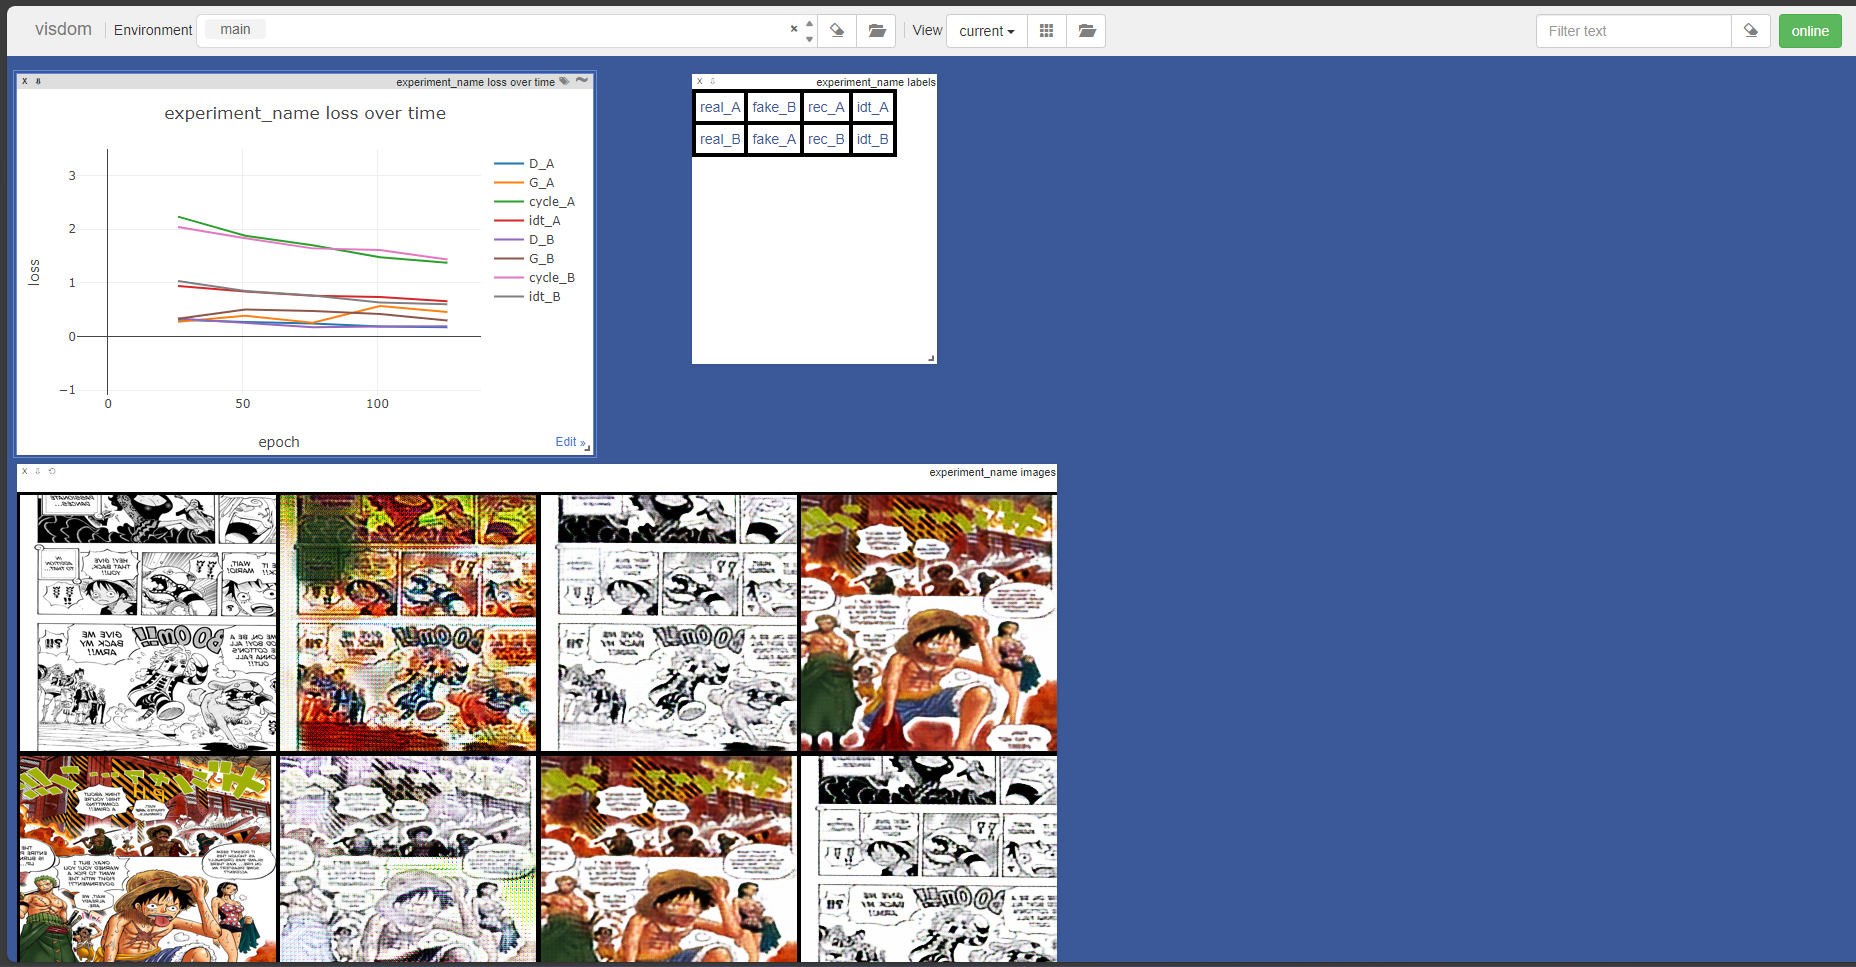
\includegraphics[width=0.8\textwidth]{img/visdom.png}
  \caption{Web-based, real-time visualization of model training and outputs}
  \label{fig:visdom}
\end{figure}

\subsubsection{User Interface}
A simple UI (figure \ref{fig:fuser_interface})has been developed using React and FastAPI for easier interaction with the model.
\begin{figure}[h!]
  \centering
  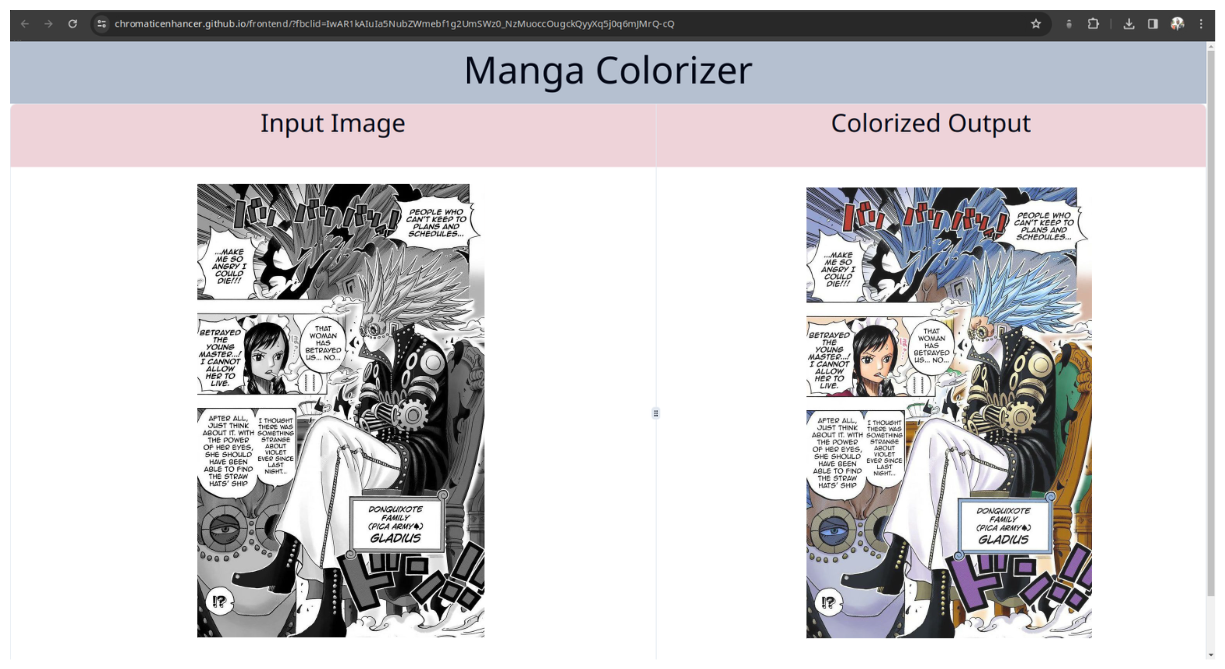
\includegraphics[width=0.8\textwidth]{img/web_interface.png}
  \caption{Demonstration of colorization via web interface}
  \label{fig:fuser_interface}
\end{figure}